\documentclass[tikz,border=10pt]{standalone}
\usepackage{tikz}
\usepackage{adjustbox}
\usepackage{fontawesome5}
\usepackage{amsmath,amssymb}
\usetikzlibrary{arrows.meta,positioning,fit,backgrounds,calc,shadows,shapes.geometric}

% Color definitions
\definecolor{lavenderDark}{RGB}{15, 44, 89}
\definecolor{lavenderDeep}{RGB}{10, 28, 58}
\definecolor{lavenderMedium}{RGB}{29, 78, 158}
\definecolor{lavenderLight}{RGB}{240, 246, 255}
\definecolor{lavenderBorder}{RGB}{180, 205, 237}
\definecolor{lavenderAccent}{RGB}{2, 132, 199}
\definecolor{prismNavy}{RGB}{15, 44, 89}
\definecolor{prismBlue}{RGB}{29, 78, 158}
\definecolor{prismTeal}{RGB}{13, 148, 136}
\definecolor{prismMint}{RGB}{236, 253, 245}
\definecolor{prismGold}{RGB}{217, 119, 6}
\definecolor{prismDark}{RGB}{15, 23, 42}
\definecolor{prismLight}{RGB}{248, 250, 252}
\definecolor{cInput}{RGB}{241, 245, 249}
\definecolor{cStem}{RGB}{224, 242, 254}
\definecolor{cStage1}{RGB}{209, 250, 229}
\definecolor{cStage2}{RGB}{254, 243, 199}
\definecolor{cStage3}{RGB}{254, 226, 226}
\definecolor{cStage4}{RGB}{207, 250, 254}
\definecolor{cHead}{RGB}{219, 234, 254}
\definecolor{cOutput}{RGB}{255, 228, 230}
\definecolor{cDeliverable}{RGB}{204, 251, 241}
\definecolor{statusFail}{RGB}{220, 38, 38}

\begin{document}
\begin{tikzpicture}[
  >=Latex,
  stagebox/.style={
    draw=lavenderDark!85,
    rounded corners=7pt,
    minimum height=7.0cm,
    text width=2.68cm,
    align=center,
    inner sep=3pt,
    line width=1.1pt,
    fill=white,
    drop shadow={shadow xshift=1.2pt, shadow yshift=-1.5pt, opacity=0.15}
  },
  pipearrow/.style={
    ->,
    draw=lavenderDark,
    line width=1.6pt,
    arrows={-Latex[length=2.8mm, width=2.0mm]}
  },
  subblk/.style={
    draw=prismNavy!85,
    rounded corners=4pt,
    fill=white,
    minimum height=1.18cm,
    text width=2.46cm,
    align=center,
    inner sep=2pt,
    line width=0.8pt,
    drop shadow={shadow xshift=0.5pt, shadow yshift=-0.5pt, opacity=0.08}
  },
  stagetitle/.style={
    text width=2.58cm,
    align=center,
    font=\fontsize{8.5}{10.5}\selectfont\bfseries,
    inner sep=2pt
  }
]

  % STAGE 1: Setup & Contract Deployment
  \node[stagebox, fill=cInput] (s1) at (0, 0) {};
  \node[stagetitle, anchor=north, text=prismNavy] at ([yshift=-6pt]s1.north) {
    \fontsize{9.5}{11.5}\selectfont\faCog\ \textbf{Stage 1}\\[2pt]
    \fontsize{7.5}{9.0}\selectfont\textbf{System Setup}\\[1pt]
    \fontsize{7.2}{8.5}\selectfont\textbf{\& Deployment}
  };
  \node[subblk, fill=white] at (0, 1.15) {\fontsize{7.8}{9.2}\selectfont\textbf{Solidity Contract}\\[2pt]\fontsize{6.8}{8.0}\selectfont Bytecode compilation\\ on EVM};
  \node[subblk, fill=white] at (0, -0.15) {\fontsize{7.8}{9.2}\selectfont\textbf{Owner Assignment}\\[2pt]\fontsize{6.8}{8.0}\selectfont \texttt{admin = msg.sender}};
  \node[subblk, fill=cStem] at (0, -1.45) {\fontsize{7.8}{9.2}\selectfont\textbf{State Init}\\[2pt]\fontsize{6.8}{8.0}\selectfont Candidate \& Voter Maps};

  % STAGE 2: Whitelisting & Registration
  \node[stagebox, fill=cStem, right=0.22cm of s1] (s2) {};
  \node[stagetitle, anchor=north, text=prismBlue] at ([yshift=-6pt]s2.north) {
    \fontsize{9.5}{11.5}\selectfont\faUserCheck\ \textbf{Stage 2}\\[2pt]
    \fontsize{7.5}{9.0}\selectfont\textbf{Whitelist}\\[1pt]
    \fontsize{7.2}{8.5}\selectfont\textbf{\& Registration}
  };
  \node[subblk, fill=white] at (s2.center |- 0, 1.15) {\fontsize{7.8}{9.2}\selectfont\textbf{Candidate Addition}\\[2pt]\fontsize{6.8}{8.0}\selectfont \texttt{addCandidate(name)}};
  \node[subblk, fill=white] at (s2.center |- 0, -0.15) {\fontsize{7.8}{9.2}\selectfont\textbf{Voter Whitelisting}\\[2pt]\fontsize{6.8}{8.0}\selectfont \texttt{registerVoter(addr)}};
  \node[subblk, fill=cHead] at (s2.center |- 0, -1.45) {\fontsize{7.8}{9.2}\selectfont\textbf{Access Control}\\[2pt]\fontsize{6.8}{8.0}\selectfont Enforced by \texttt{onlyAdmin}};

  % STAGE 3: Wallet Authentication
  \node[stagebox, fill=cStage2!50, right=0.22cm of s2] (s3) {};
  \node[stagetitle, anchor=north, text=prismGold!90!black] at ([yshift=-6pt]s3.north) {
    \fontsize{9.5}{11.5}\selectfont\faKey\ \textbf{Stage 3}\\[2pt]
    \fontsize{7.5}{9.0}\selectfont\textbf{Wallet}\\[1pt]
    \fontsize{7.2}{8.5}\selectfont\textbf{Authentication}
  };
  \node[subblk, fill=white] at (s3.center |- 0, 1.15) {\fontsize{7.8}{9.2}\selectfont\textbf{MetaMask Connect}\\[2pt]\fontsize{6.8}{8.0}\selectfont \texttt{connect()} Handshake};
  \node[subblk, fill=white] at (s3.center |- 0, -0.15) {\fontsize{7.8}{9.2}\selectfont\textbf{Address Check}\\[2pt]\fontsize{6.8}{8.0}\selectfont \texttt{voters[addr].isReg}};
  \node[subblk, fill=cStage2] at (s3.center |- 0, -1.45) {\fontsize{7.8}{9.2}\selectfont\textbf{ECDSA Verify}\\[2pt]\fontsize{6.8}{8.0}\selectfont secp256k1 Non-repudiation};

  % STAGE 4: Ballot & Double-Voting Mitigation
  \node[stagebox, fill=cStage3!40, right=0.22cm of s3] (s4) {};
  \node[stagetitle, anchor=north, text=statusFail!90!black] at ([yshift=-6pt]s4.north) {
    \fontsize{9.5}{11.5}\selectfont\faLock\ \textbf{Stage 4}\\[2pt]
    \fontsize{7.5}{9.0}\selectfont\textbf{Ballot \& Double}\\[1pt]
    \fontsize{7.2}{8.5}\selectfont\textbf{Vote Mitigation}
  };
  \node[subblk, fill=white] at (s4.center |- 0, 1.15) {\fontsize{7.8}{9.2}\selectfont\textbf{Candidate Pick}\\[2pt]\fontsize{6.8}{8.0}\selectfont Selection on \texttt{voting.html}};
  \node[subblk, fill=white] at (s4.center |- 0, -0.15) {\fontsize{7.8}{9.2}\selectfont\textbf{Atomic Acceptance}\\[2pt]\fontsize{6.8}{8.0}\selectfont $\text{Accept} = 1 \iff \neg\text{voted}$};
  \node[subblk, fill=cStage3] at (s4.center |- 0, -1.45) {\fontsize{7.8}{9.2}\selectfont\textbf{State Mutation}\\[2pt]\fontsize{6.8}{8.0}\selectfont \texttt{voted=true; tally++}};

  % STAGE 5: Consensus & Results Audit
  \node[stagebox, fill=cStage1!50, right=0.22cm of s4] (s5) {};
  \node[stagetitle, anchor=north, text=prismTeal!90!black] at ([yshift=-6pt]s5.north) {
    \fontsize{9.5}{11.5}\selectfont\faCheckCircle\ \textbf{Stage 5}\\[2pt]
    \fontsize{7.5}{9.0}\selectfont\textbf{Consensus \&}\\[1pt]
    \fontsize{7.2}{8.5}\selectfont\textbf{Result Audit}
  };
  \node[subblk, fill=white] at (s5.center |- 0, 1.15) {\fontsize{7.8}{9.2}\selectfont\textbf{PoA Block Sealing}\\[2pt]\fontsize{6.8}{8.0}\selectfont $H(B_i) = \text{SHA-256}(\dots)$};
  \node[subblk, fill=white] at (s5.center |- 0, -0.15) {\fontsize{7.8}{9.2}\selectfont\textbf{Event Emission}\\[2pt]\fontsize{6.8}{8.0}\selectfont \texttt{emit VoteCast(\dots)}};
  \node[subblk, fill=cDeliverable] at (s5.center |- 0, -1.45) {\fontsize{7.8}{9.2}\selectfont\textbf{Real-Time Audit}\\[2pt]\fontsize{6.8}{8.0}\selectfont Public Tally $N(c)$ live};

  % Connectors
  \draw[pipearrow] (s1) -- (s2);
  \draw[pipearrow] (s2) -- (s3);
  \draw[pipearrow] (s3) -- (s4);
  \draw[pipearrow] (s4) -- (s5);

\end{tikzpicture}
\end{document}
